
\chapter{Rezultati} % Main chapter title

\label{Rezultati} % For referencing 

Od ukupno 186 MF ključnih reči sa preko 20 pridruženih proteina, 116 su
statistički značajne od čega su 53 uređene (p<0.05), a 63 neuređene (p>0.95).
Od ukupno 1781 MF termina sa preko 20 pridruženih proteina (dobijeno
grupisanjem), 1315 su statistički značajni od čega su 699 uređeni, a 616
neuređeni.  Tabela \ref{tab:kw_uopsteno} prikazuje razlike u odnosu na
originalne rezultate.

\begin{table}[htpb]
\begin{tabular}{|r|c|c|c|}
  \hline
             & Org. rez.  & \multicolumn{2}{c|}{ Naši rezultati} \\
             & Xie2007 kw & MF kw  & MF termini \\
  \hline                             
  ukupno     & 143        & 186      & 1781      \\
  p<0.05 (uređene)    & 37         & 53       & 699     \\ 
  p>0.95 (neuređene)    & 51         & 63       & 616     \\
  \hline
\end{tabular}
  \centering
  \caption{Uopšteno poređenje rezultata}
  \label{tab:kw_uopsteno}
\end{table}


Pošto su izvršene dve vrste grupisanja rezultati će biti predstavljeni na
sledeći način. Tabelama \ref{fig:KWtop20dis} i \ref{fig:KWtop20ord} prikazano
je poređenje originalnih rezultata sa našim grupisanjem po \keyword{ključnim
rečima}. Navedene tabele sortirane su po Z-skor vrednosti.  Za razliku od
originalnih rezultata, naše tabele ne sadrže broj klastera, ali dodatno sadrže 
informaciju o procentu neuređenih proteina $F_j$ koju nazivamo
\keyword{neuređenost funkcije}. 

Grupisanje po ključnim rečima predstavlja se kao podgraf originalne MF
ontologije pri čemu su zadržani samo statistički značajni termini.  Isečak
grafa neuređenih termina prikazan je na Slici \ref{fig:disorder_example}.
Pozadinska boja termina kodira pomenutu neuređenost termina. Korišćeno je
viridis \cite{viridis} mapiranje boja koje nulu predstavlja tamno ljubičastom a
jedinicu svetlo žutom. Tamni, plavkasti termini su uređeni dok su svetli,
zelenkasti neuređeni. Crvene elipse predstavljaju najznačajnijih 20 (ne)uređenih ključnih
reči iz originalnog rada i povezani su sa terminima preko četiri tipa veze.
Zelena veza predstavlja direktno mapirnaje, crvena preko imena, ljubičasta
preko sinonima, a žuta pominjanje u definiciji.  Na adresi \cite{rezultati} u
\file{.svg} formatu dostupni su svi rezultati ovoga oblika. 
Pomenute slike, ukoliko se otvore u veb pretraživaču, prikazuju dodatne
informacije o terminima iznad kojih je pozicionirana strelica miša.  Svaki
termin sadrži odgovarajući hiperlink ka \textit{AmiGO}\footnote{\textit{AmiGO}
je skup alat za pretraživanje i prikazivanje GO termina } veb stranici.

Radi izbegavanja dvosmislenosti u daljem tekstu, imena ključnih reči imaće
dodeljen prefiks \textit{KW: } dok će imena MF termina imati prefiks
\textit{MF: }.

\clearpage

\begin{figure}[th]
\hspace*{-2.5cm} 
\includegraphics[angle=0, scale=0.45]{Figures/plots/KWtop20dis.pdf}
\decoRule
\caption {
  20 statistički najznačajnijih \keyword{neuređenih} ključnih reči iz rada
  \parencite{Xie2007} upoređeno sa našom analizom po ključnim rečima nad CAFA3 podacima.
}
\label{fig:KWtop20dis}
\end{figure}

\begin{figure}[th]
\hspace*{-2.5cm} 
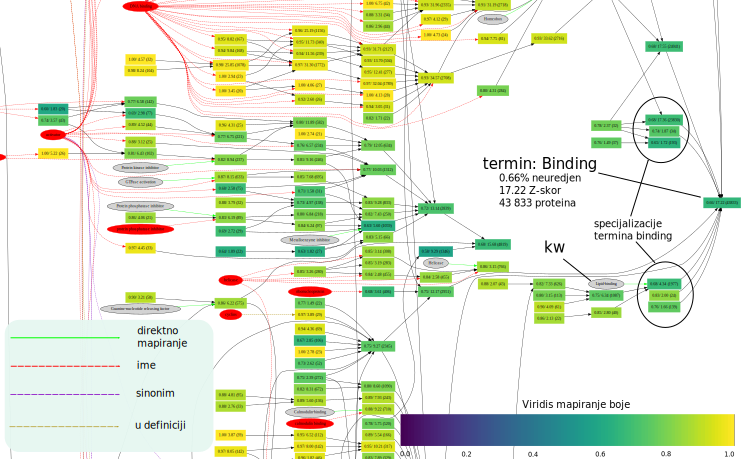
\includegraphics[angle=0, scale=0.9]{Figures/plots/disorder_example.pdf}
\decoRule
\caption {
  Isečak grafa neuređenih termina
}
\label{fig:disorder_example}
\end{figure}



\subsection{Poređenje neuređenih funkcija}

% Slika \ref{fig:KWtop20dis} prikazuje originlne rezultate 20 najznačajnijih neuređenih
% ključnih reči molekulske funkcije sortirane po Z-skoru (levo) i njihovo mapiranje
% na ponovljenu analizu nad CAFA3 proteina dužih od 40AK  grupisanih po \keyword{ključnim rečima} (desno).
% Korišćen je standardni $P_L$ model.


1. \kw{Ribonucleoprotein} nalazi se na 7. mestu, ima  Z-skor 13.39 (skoro duplo manje) i neuređenosti 0.6.
Direktno mapiranje nije nađeno. Pronađeni \mf{Ribonucleoprotein binding complex}
ima Z-skor od svega 3.51, neuređenost 0.68 obuhvatajući svega 406 proteina.

2. \kw{Ribosomal protein} nalazi se na 10. mestu, ima Z-skor 9.34 (duplo manje) i neuređenost 0.53.
Direkto mapiranje nije nađeno. Pronađen je sinonim u širem smislu,
\mf{structual costituent of ribosome} sa skoro istim karakteristikam Z-skor 9.79 i neuređenost 0.53.

3. \kw{Developmental protein} nalazi se na 2. mestu, ima Z-skor 31.1 i neuređenost 0.87.
\keyword{MF Mapiranje nije nađeno!}

4. \kw{Hormone} se nalazi na 14. mestu, ima Z-skor 7.24 (duplo manji) i neuređenost 0.59.
Direktno mapiran \mf{Hormone activity} ima Z-skor 8.93 neuređenost 0.61.
Dodatni relevantni MF termini uključuju:
\begin{itemize}
  \item \mf{Hormone receptor binding} Z-skor 8.4, neuređenost 0.84 
  \item \mf{Steroid Hormone receptor binding} Z-skor 9.4, neuređenost 0.92 
  \item \mf{Nuclear Hormone receptor binding} Z-skor 9.07, neuređenost 0.9 
  \item \mf{Thyroid Hormone receptor binding} Z-skor 9.07, neuređenost 0.9 
  \item \mf{Nuclear Hormone receptor activity} Z-skor 4.31, neuređenost 1.0 
\end{itemize}


5. \kw{Growth factor} nalazi se na 11. mestu, ima Z-skor 8.98 i neuređenost 0.7.
Direktno mapiran \mf{Growth factor activity} ima Z-skor 9.2 i neuređenost 0.7.
Dodatna mapiranja uključuju:
\begin{itemize}
  \item \mf{Growth factor receptor binding} ima Z-skor 3.76 i neuređenost 0.66.
    Postoji nekoliko specijalizacije ovog termina koje imaju veći Z-skor i neuređenost.
  \item \mf{Growth factor binding} ima Z-skor 4.42 i neuređenost 0.79. Postoji
    nekoliko specijalizacija visoke neuređenosti pogotovo za
    \textit{insulin-like growth factor} vezivanje.
\end{itemize}


6. \kw{Cytokine} nije statistički značajan u našoj analizi ključnih reči.
\mf{Cytokine receptor binding} ima Z-skor 2.57 (4 puta manje) i neuređenost 0.56

7. \kw{Neuropeptide} nalazi se na 20. mestu, ima Z-skor 6 i neređenost 0.68.
Direktno mapiranje nije nađeno.
\mf{neuropeptide receptor binding} ima Z-skor 6.71 i neuređenost 0.73 dok,
\mf{neuropeptide hormone activity} ima Z-skor 6.06 i neuređenost 0.65.


8. \kw{Activator} nalazi se na 11. mestu, ima Z-skor 28.12 (3 put veći) i neuređenost 0.88.
\\ Ekvivalentan MF termin ne postoji.
% Potencijalno povezani MF termini:
% \begin{itemize}
%   \item \mf{enzyme activator activity}
%   \item \mf{MAP kinase kinase activator} 
% \end{itemize}


9. \kw{GAP protein} je izbačen iz analize jer sadrži manje od 20 proteina.

10. \kw{Antigen} je izbačena iz novih verzija ključnih reči.
Analizom definicije \mf{MHC class II protein binding} zaključena je relavantnost
u kontekstu antigena (iterakcija sa \textit{histocompatibility} kompleksima).
Z-skor 2.26, neuređenost 0.85. Ova funkcija sadrži svega 20 proteina.

11. \kw{Repressor} nalazi se na 4. mestu, ima Z-skor 22.63 (skoro 4 puta veća) i neuređenost 0.85.
\\ Ekvivalentan MF termin ne postoji.


12. \kw{Chromatin regulator} nalazi se na 6. mestu, ima Z-skor 13.91 (duplo veća) i neuređenost 0.9.
\\ Odgovarajući termin \mf{covalent chromatin modification} nema dovoljno pridruženih proteina.

13. \kw{Pyrogen} je izbačen iz analize jer sadrži manje od 20 proteina.

14. \kw{Vasoactive} nalazi se na 26. mestu, ima Z-skor 4.3 (orig. 5.56) i neuređenost 0.76.
\\ Odgovarajući \mf{regulation of blood vessel size} nema dovoljno pridruženih proteina.

15. \kw{Amphibian defense peptide} nalazi se na 31. mestu, ima Z-skor 3.34 (orig. 5.44) i neuređenost 0.53.
\\ Odgovarajući \mf{defense response} nema dovoljno pridruženih proteina.

16. \kw{GTPase activation} nalazi se na 18. mestu, ima Z-skor 6.28 (orig. 5.44) i neuređenost 0.88.
Direktno mapiran \mf{GTPase activation} ima Z-skor 8.06, neuređenost 0.87.

17. \kw{Endorphin} nalazi se na 30. mestu, ima Z-skor 3.49 i neuređenost 1.0.
\\ Odgovarajući \mf{neuropeptide signaling pathway} nema dovoljno pridruženih proteina. Sa druge strane vezivanje neuropeptida je pristuno 

18. \kw{Opioid peptide} nalazi se na 33. mestu, ima Z-skor 3.14 i neuređenost 1.0.
Direktno mapiran \mf{Opioid peptide binding } Nije statistički značajan.

19. \kw{Protein phosphatase inhibitor} nalazi se na 23. mestu, ima Z-skor 5.07 i neuređenost 0.81.
Direktno mapiranje \mf{Protein phosphatase inhibitor activity} ima Z-skor 5.62 i neurđenost 0.83.

20. \kw{Cyclin} nalazi se na 15. mestu, ima Z-skor 7.18 i neuređenost 0.87.
Direktno mapirnaje nije nađeno.
\mf{Cyclin binding} ima Z-skor 2.042 i neuređenost 0.71.


\subsection{ Neuređene ključne reči značajne samo za CAFA3 podatke}

1. \kw{DNA-binding} ima Z-skor 46.9 i neuređenost 0.87.
Mapiran {DNA binding} ima Z-skor 46.13 i neurđenost 0.86.
Pored ovog postoje mnogi specijalizovani neuređeni termini

5. \kw{RNA-binding} ima Z-skor 16.62 i neuređenost 0.76.
Direktno mapiran {RNA binding} ima Z-skor 19.79 i neurđenost 0.73.
Pored ovog postoje mnogi specijalizovani neuređeni termini

8. \kw{Serine/threonine-protein kinase} ima Z-skor 11.56 i neuređenost 0.84.
Direktno mapiran {proein serine/threonine kinase activity} ima Z-skor 12.88 i neurđenost 0.84.

9. \kw{Chaperone} ima Z-skor 10.02 i neuređenost 0.71.
Nema direktno mapiranje ali su pronađeni:
\begin{itemize}
  \item \mf{chaperone binding} ima Z-skor 8.86 i neuređenost 0.84.
  \item \mf{ufolded protein binding} sinonima ima Z-skor 8.86 i neuređenost 0.84 (mapiran preko nekolio šest \textit{related} sinonima).
\end{itemize}

12. \kw{Protein kinase inhibitor} ima Z-skor 8.34 i neuređenost 0.96.
Direktno mapiran \mf{protein kinase inhibitor activity} ima Z-skor 8.94 i neuređenost 0.82.

13. \kw{Calmodulin-binding} ima Z-skor 7.57 i neuređenost 0.9.
Direktno mapiran \mf{calmodulin binding} ima Z-skor 9.22 i neuređenost 0.88.

16. \kw{Signal transduction inhibitor} ima Z-skor 6.76 i neuređenost 0.84.
\\ Odgovarajući \mf{negative regulation of signal transduction} nema dovoljno pridruženih proteina.

17. \kw{Guanine-nucleotide releasing factor} ima Z-skor 6.4 i neuređenost 0.96.
Direktno mapiran \mf{guanyl-nucleotide exchange factor activity} ima Z-skor 6.22 i neuređenost 0.86.

19. \kw{Growth factor binding} ima Z-skor 6.09 i neuređenost 1.00.
\mf{Growth factor binding} ima Z-skor 4.42 i neuređenost 0.79. Postoji
nekoliko specijalizacija visoke neuređenosti pogotovo za
\textit{insulin-like growth factor} vezivanje.



\subsection{Poređenje uređenih funkcija}




\subsection{ Neuređene ključne reči značajne samo za CAFA3 podatke}



\begin{figure}[th]
\centering
\hspace*{-2.0cm} 
\includegraphics[angle=0, scale=0.45]{Figures/plots/KWtop20ord.pdf}
\decoRule
\caption {
  20 statistički najznačajnijih \keyword{uređenih} ključnih reči iz rada
  \parencite{Xie2007} upoređeno sa našom analizom po ključnim rečima nad CAFA3 podacima.
}
\label{fig:KWtop20ord}
\end{figure}



\subsection{$P_L random$ model}

\begin{figure}[th]
\centering
\includegraphics[scale=0.32]{Figures/plots/KW_random.pdf}
\decoRule
\caption {
  $P_L$ levo, upoređen sa $P_L random$ desno dobijeno iz CAFA3 proteina grupisanih po ključnim rečima.
}
\label{fig:KW_random}
\end{figure}
